
\section{Method}\label{sec:method}


In this section, we describe our new problem setting in CL where historical data are available while the processing time is limited when learning new tasks. To this end, we present our method for learning replay schedules in CL where the idea is to learn schedules of which tasks the network should replay at different times. 
%In this section, we describe our method for learning replay schedules in CL. The idea is to learn schedules of which tasks %memory examples 
%the network should replay at different times. 
We use Monte Carlo tree search (MCTS)~\citep{coulom2006efficient} to learn a scheduling policy by encouraging searches for promising replay schedules based on the classification accuracy. 


\subsection{Problem Setting}\label{paperC:sec:problem_setting}

We focus on a slightly new setting, considering the needs for CL in the real-world where all historical data can be available since data storage is cheap. 
However, as this data volume is typically huge, we are often prohibited from replaying all historical data due to processing time constraints. 
Therefore, the goal is to determine which historical tasks to revisit and sample a small replay memory from the selected tasks to mitigate catastrophic forgetting as efficiently as possible. 

\setlength{\abovedisplayskip}{0pt}
\setlength{\belowdisplayskip}{0pt}
\setlength{\abovedisplayshortskip}{0pt}
\setlength{\belowdisplayshortskip}{0pt}

Here, we introduce the notation of our problem setting which resembles the traditional CL setting for image classification. We let a neural network $f_{\vtheta}$, parameterized by $\vtheta$, learn $T$ tasks sequentially from the datasets $\gD_1, \dots, \gD_T$ arriving one at a time. 
The $t$-th dataset $\gD_t = \{(\vx_{t}^{(i)}, y_{t}^{(i)})\}_{i=1}^{N_{t}}$ consists of $N_t$ samples where $\vx_{t}^{(i)}$ and $y_{t}^{(i)}$ are the $i$-th data point and class label respectively. The training objective at task $t$ is given by 
\begin{align}
	\underset{\vtheta}{\text{min}} \sum_{i=1}^{N_t} \ell(f_{\vtheta}(\vx_t^{(i)}), y_{t}^{(i)}),
\end{align}
where $\ell(\cdot)$ is the loss function, e.g., cross-entropy loss in our case. 
When learning task $t$, the network $f_{\vtheta}$ is at risk of catastrophically forgetting the previous $t-1$ tasks. Next, we describe our method for constructing this replay memory.  

We assume that historical data from old tasks are accessible at any time step $t$. 
However, due to processing time constraints, we can only fill a small replay memory $\gM$ with $M$ historical samples for replay. 
The challenge then becomes how to select the $M$ replay samples to efficiently retain knowledge of old tasks. We focus on selecting the samples on task-level by deciding on the task proportion $(p_1, \dots, p_{t-1})$ of samples to fetch from each task, where $p_{i} \geq 0$ is the proportion of $M$ samples from task $i$ to place in $\gM$ and $\sum_{i=1}^{t-1} p_i = 1$. To simplify the selection of which tasks to replay, we construct a discrete set of possible task proportions that can be used for constructing $\gM$.



 %%% RS-MCTS EXAMPLE FIGURE 
\begin{figure*}[t]
\centering 
\setlength{\figwidth}{.77\textwidth}
\setlength{\figheight}{.3\textheight}
\definecolor{color0}{rgb}{0.945098039215686,0.435294117647059,0.125490196078431}
\definecolor{color1}{rgb}{0.843137254901961,0.6,0.133333333333333}
\definecolor{color2}{rgb}{0.250980392156863,0.337254901960784,0.631372549019608}
\definecolor{color3}{rgb}{1,0.498039215686275,0}
\definecolor{color4}{rgb}{0.94509803921,0.23529411764,0.12549019607}
\definecolor{color5}{rgb}{0.94509803921,0.23529411764,0.12549019607}

\resizebox{0.95\textwidth}{!}{
\begin{tikzpicture}[
    roundnode/.style={circle, draw=color3, text=color3, very thick, minimum size=7mm},
    squarednode/.style={rectangle, draw=black, fill=white, text=black, very thick, minimum size=7mm, align=center, rounded corners},
    %tasknode/.style={rectangle, draw=blue!50, fill=blue!10, text=black, very thick, minimum size=7mm, align=center, depth=2cm, rounded corners},
    %task/.style={rectangle, rounded corners, thick,inner sep=3pt},
    ]
    %%% Task 1 level
    \draw[draw=blue!50, fill=blue!10, very thick, rounded corners] (0,0) rectangle (16,-2);
    \node[squarednode] (dataset1) at (1.,-1) { \textbf{Task 1} \\ 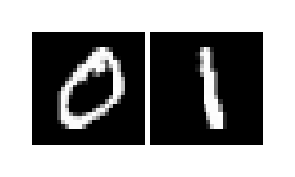
\includegraphics[width=0.08\textwidth]{PaperC/figures/mcts_tikz/dataset_two_images/dataset1.eps}};
    \node[squarednode] (v1) at (9,-1) {\large $\emptyset$};
    
    %%% Task 2 level
    \draw[draw=red!50, fill=red!10, very thick, rounded corners] (0,-2) rectangle (16,-4);
    
    \node[squarednode] (dataset2) at (1.,-3) { \textbf{Task 2} \\ 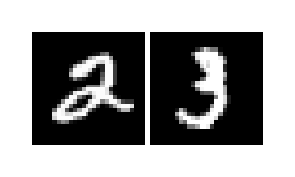
\includegraphics[width=0.08\textwidth]{PaperC/figures/mcts_tikz/dataset_two_images/dataset2.eps}};
    \node[squarednode, text=color3] (v2) at (9,-3) {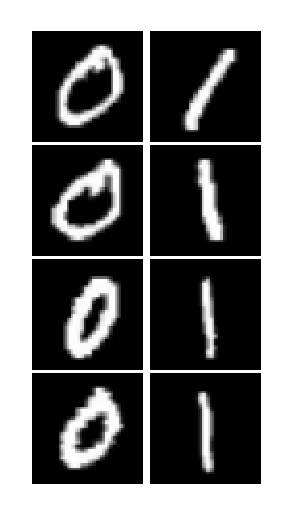
\includegraphics[width=0.045\textwidth]{PaperC/figures/mcts_tikz/vertical_rs/task1_only.eps}};
    \draw[<-] (v2) -- (v1);
    
    %%% Task 3 level
    \draw[draw=color3!50, fill=color3!10, very thick, rounded corners] (0,-4) rectangle (16,-6);
    \node[squarednode] (dataset3) at (1.,-5) { \textbf{Task 3} \\ 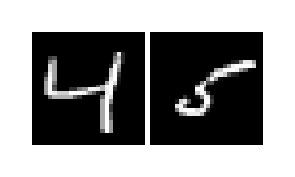
\includegraphics[width=0.08\textwidth]{PaperC/figures/mcts_tikz/dataset_two_images/dataset3.eps}};
    \node[squarednode, text=color3] (v3_beg) at (5,-5) {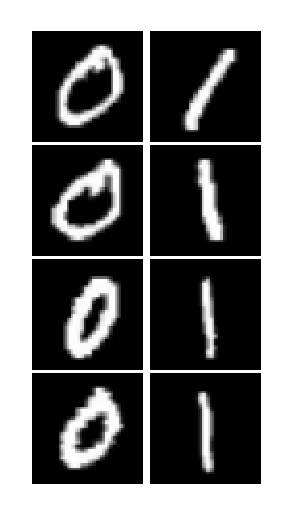
\includegraphics[width=0.045\textwidth]{PaperC/figures/mcts_tikz/vertical_rs/task1_only.eps}};
    \draw[<-, blue, very thick] (v3_beg) -- (v2);
    
    \node[squarednode, text=color3] (v3_mid) at (9,-5) {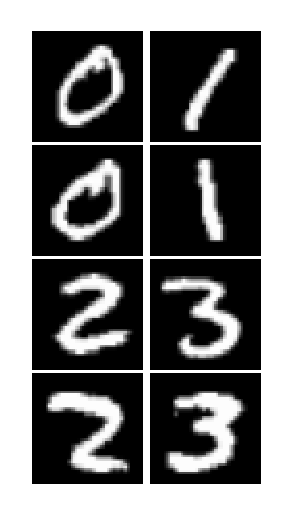
\includegraphics[width=0.045\textwidth]{PaperC/figures/mcts_tikz/vertical_rs/equal_task3.eps}};
    \draw[<-, red, very thick] (v3_mid) -- (v2);
    
    \node[squarednode, text=color3] (v3_end) at (13,-5) {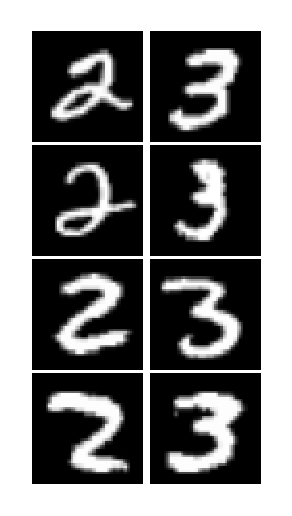
\includegraphics[width=0.045\textwidth]{PaperC/figures/mcts_tikz/vertical_rs/task2_only.eps}};
    \draw[<-, purple, very thick] (v3_end) -- (v2);
    
    %%% Task 4 level
    \draw[draw=magenta!50, fill=magenta!10, very thick, rounded corners] (0,-6) rectangle (16,-8);
    
    \node[squarednode] (dataset4) at (1.,-7) { \textbf{Task 4} \\ 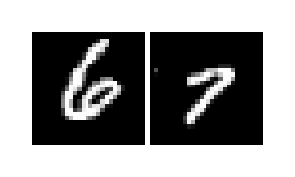
\includegraphics[width=0.08\textwidth]{PaperC/figures/mcts_tikz/dataset_two_images/dataset4.eps}};
    
    \node[squarednode, text=color3] (v41_beg) at (4,-7) {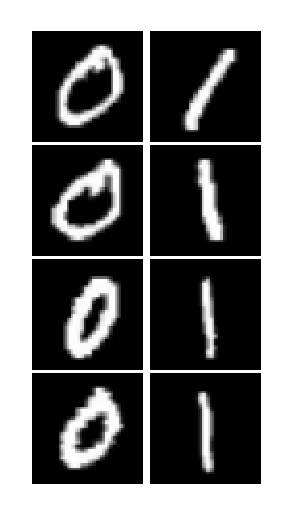
\includegraphics[width=0.045\textwidth]{PaperC/figures/mcts_tikz/vertical_rs/task1_only.eps}};
    \draw[<-, blue, very thick] (v41_beg) -- (v3_beg);
    %\draw[<-] (v4_beg) -- (v3_mid);
    %\draw[<-] (v4_beg) -- (v3_end);
    
    \node[] (v41_dots) at (5,-7) {\large $\cdots$};
    %\draw[<-] (v4_dots1) -- (v3_beg);%\draw[<-, dashed] (v4_dots1) -- (v3_beg);
    %\draw[<-] (v4_dots1) -- (v3_mid);
    %\draw[<-] (v4_dots1) -- (v3_end);
    
    \node[squarednode, text=color3] (v41_end) at (6,-7) {\includegraphics[width=0.045\textwidth]{PaperC/figures/mcts_tikz/vertical_rs/task3_only.eps}};
    \draw[<-] (v41_end) -- (v3_beg);
    
    \node[squarednode, text=color3] (v42_beg) at (7.1,-7) {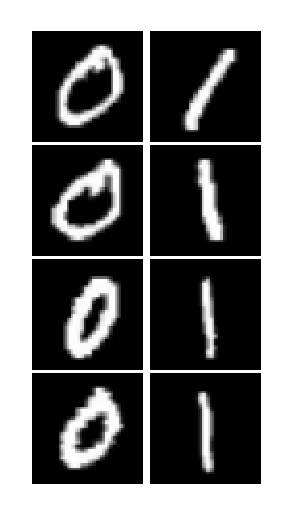
\includegraphics[width=0.045\textwidth]{PaperC/figures/mcts_tikz/vertical_rs/task1_only.eps}};
    \draw[<-] (v42_beg) -- (v3_mid);
    
    \node[] (v42_dots1) at (8,-7) {\large $\cdots$};
    
    \node[squarednode, text=color3] (v42_mid) at (9,-7) {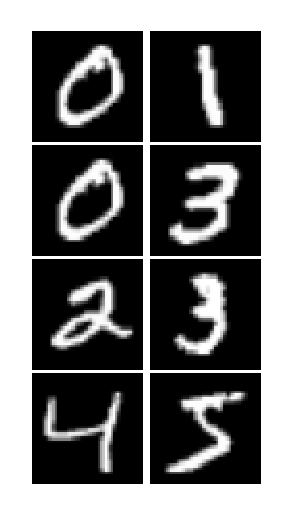
\includegraphics[width=0.045\textwidth]{PaperC/figures/mcts_tikz/vertical_rs/equal_task4.eps}};
    \draw[<-, red, very thick] (v42_mid) -- (v3_mid);
    
    \node[] (v42_dots2) at (10,-7) {\large $\cdots$};
    
    \node[squarednode, text=color3] (v42_end) at (11,-7) {\includegraphics[width=0.045\textwidth]{PaperC/figures/mcts_tikz/vertical_rs/task3_only.eps}};
    \draw[<-] (v42_end) -- (v3_mid);
    %\node[squarednode, text=color3] (v4_end1) at (6.5,-7) {\includegraphics[width=0.08\textwidth]{PaperC/figures/mcts_tikz/replay_batches/task3_only.eps}};
    %\draw[<-] (v4_end1) -- (v3_beg);
    
    \node[squarednode, text=color3] (v43_beg) at (12.1,-7) {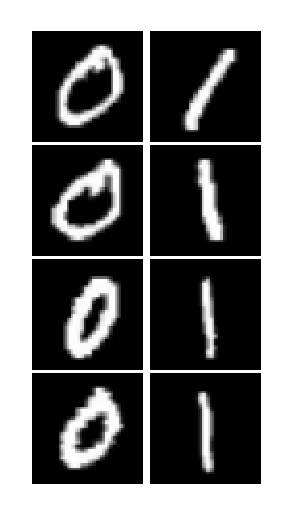
\includegraphics[width=0.045\textwidth]{PaperC/figures/mcts_tikz/vertical_rs/task1_only.eps}};
    \draw[<-] (v43_beg) -- (v3_end);
    
    \node[] (v43_dots) at (13,-7) {\large $\cdots$};
    %\draw[<-] (v4_dots2) -- (v3_beg);
    %\draw[<-] (v4_dots2) -- (v3_mid);
    %\draw[<-] (v4_dots2) -- (v3_end);
    
    \node[squarednode, text=color3] (v43_end) at (14,-7) {\includegraphics[width=0.045\textwidth]{PaperC/figures/mcts_tikz/vertical_rs/task3_only.eps}};
    \draw[<-, purple, very thick] (v43_end) -- (v3_end);
    %\draw[<-] (v4_end) -- (v3_mid);
    %\draw[<-, purple, very thick] (v4_end) -- (v3_end);


    %%% Task 5 level
    \draw[draw=green!50, fill=green!10, very thick, rounded corners] (0,-8) rectangle (16,-10);
    \node[squarednode] (dataset5) at (1.,-9) { \textbf{Task 5} \\ 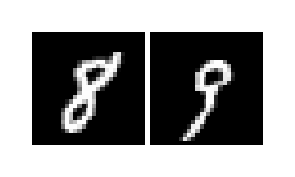
\includegraphics[width=0.08\textwidth]{PaperC/figures/mcts_tikz/dataset_two_images/dataset5.eps}};
    
    \node[squarednode, text=color3] (v51_beg) at (3,-9) {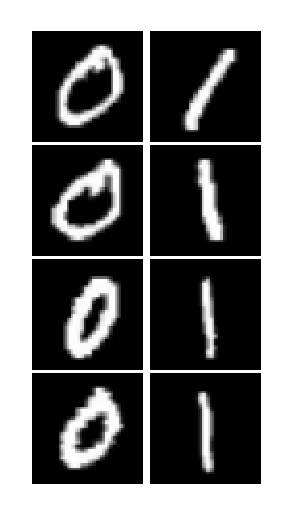
\includegraphics[width=0.045\textwidth]{PaperC/figures/mcts_tikz/vertical_rs/task1_only.eps}};
    \draw[<-, blue, very thick] (v51_beg) -- (v41_beg);
    %\draw[<-] (v5_beg) -- (v4_dots1);
    %\draw[<-] (v5_beg) -- (v4_mid);
    %\draw[<-] (v5_beg) -- (v4_dots2);
    %\draw[<-] (v5_beg) -- (v4_end);
    
    \node[] (v51_dots) at (4,-9) {\large $\cdots$};
    %\draw[<-] (v5_dots1) -- (v4_beg1);
    %\draw[<-] (v5_dots1) -- (v4_dots1);
    %\draw[<-] (v5_dots1) -- (v4_mid);
    %\draw[<-] (v5_dots1) -- (v4_dots2);
    %\draw[<-] (v5_dots1) -- (v4_end);
    
    \node[squarednode, text=color3] (v51_end) at (5,-9) {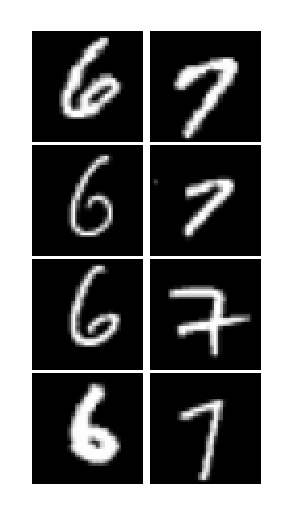
\includegraphics[width=0.045\textwidth]{PaperC/figures/mcts_tikz/vertical_rs/task4_only.eps}};
    \draw[<-] (v51_end) -- (v41_beg);
    
    %\node[squarednode, text=color3] (v52_beg) at (5,-9) {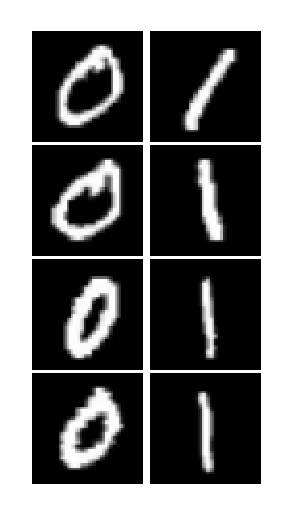
\includegraphics[width=0.045\textwidth]{PaperC/figures/mcts_tikz/vertical_rs/task1_only.eps}};
    
    %\node[squarednode, text=color3] (v5_mid_low) at (6,-9) {\includegraphics[width=0.06\textwidth]{PaperC/figures/mcts_tikz/replay_batches/task5_middle0.eps}};
    %\draw[<-] (v5_mid_low) -- (v4_beg);
    %\draw[<-] (v5_mid_low) -- (v4_dots1);
    %\draw[<-] (v5_mid_low) -- (v4_mid);
    %\draw[<-] (v5_mid_low) -- (v4_dots2);
    %\draw[<-] (v5_mid_low) -- (v4_end);
    
    \node[] (v52_dots) at (6,-9) {\large $\cdots$};
    \draw[<-, dashed] (v52_dots) -- (v41_end);
    
    \node[] (v53_dots) at (7.1,-9) {\large $\cdots$};
    \draw[<-, dashed] (v53_dots) -- (v42_beg);
    
     \node[] (v54_dots) at (8,-9) {\large $\cdots$};
    %\draw[<-] (v5_dots2) -- (v4_beg);
    %\draw[<-] (v5_dots2) -- (v4_dots1);
    %\draw[<-] (v5_dots2) -- (v4_mid);
    %\draw[<-] (v5_dots2) -- (v4_dots2);
    %\draw[<-] (v5_dots2) -- (v4_end);
    
    \node[squarednode, text=color3] (v52_mid) at (9,-9) {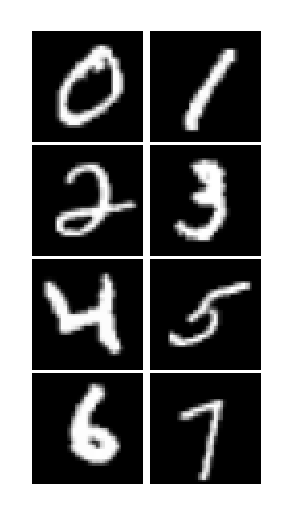
\includegraphics[width=0.045\textwidth]{PaperC/figures/mcts_tikz/vertical_rs/equal_task5.eps}};
    \draw[<-, red, very thick] (v52_mid) -- (v42_mid);
    %\draw[<-] (v5_mid) -- (v4_beg);
    %\draw[<-] (v5_mid) -- (v4_dots1);
    %\draw[<-, red, very thick] (v5_mid) -- (v4_mid);
    %\draw[<-] (v5_mid) -- (v4_dots2);
    %\draw[<-] (v5_mid) -- (v4_end);
    
    \node[] (v55_dots) at (10,-9) {\large $\cdots$};
    
    \node[] (v56_dots) at (11,-9) {\large $\cdots$};
    \draw[<-, dashed] (v56_dots) -- (v42_end);
    
    \node[] (v57_dots) at (12.1,-9) {\large $\cdots$};
    \draw[<-, dashed] (v57_dots) -- (v43_beg);
    %\draw[<-] (v5_dots3) -- (v4_beg);
    %\draw[<-] (v5_dots3) -- (v4_dots1);
    %\draw[<-] (v5_dots3) -- (v4_mid);
    %\draw[<-] (v5_dots3) -- (v4_dots2);
    %\draw[<-] (v5_dots3) -- (v4_end);
    
    %\node[squarednode, text=color3] (v5_mid_high) at (12,-9) {\includegraphics[width=0.06\textwidth]{PaperC/figures/mcts_tikz/replay_batches/task5_middle1.eps}};
    %\draw[<-] (v5_mid_high) -- (v4_beg);
    %\draw[<-] (v5_mid_high) -- (v4_dots1);
    %\draw[<-] (v5_mid_high) -- (v4_mid);
    %\draw[<-] (v5_mid_high) -- (v4_dots2);
    %\draw[<-] (v5_mid_high) -- (v4_end);
    
    \node[squarednode, text=color3] (v53_beg) at (13,-9) {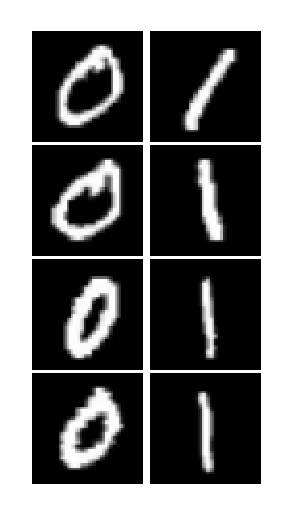
\includegraphics[width=0.045\textwidth]{PaperC/figures/mcts_tikz/vertical_rs/task1_only.eps}};
    \draw[<-] (v53_beg) -- (v43_end);
    
    \node[black] (v58_dots) at (14,-9) {\large $\cdots$};
    
    %\draw[--, dashed] (v5_dots4) -- (v43_dots);
    %\draw[<-] (v5_dots4) -- (v4_mid);
    %\draw[<-] (v5_dots4) -- (v4_dots2);
    %\draw[<-] (v5_dots4) -- (v4_end);
    
    \node[squarednode, text=color3] (v53_end) at (15,-9) {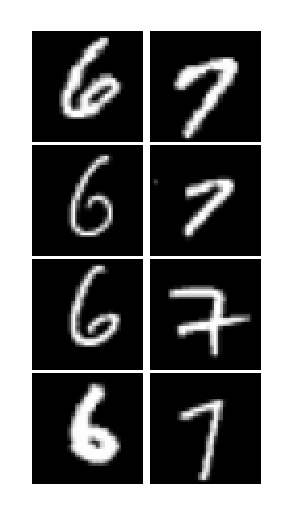
\includegraphics[width=0.045\textwidth]{PaperC/figures/mcts_tikz/vertical_rs/task4_only.eps}};
    \draw[<-, purple, very thick] (v53_end) -- (v43_end);
    %\draw[<-] (v5_end) -- (v4_beg);
    %\draw[<-] (v5_end) -- (v4_dots1);
    %\draw[<-] (v5_end) -- (v4_mid);
    %\draw[<-] (v5_end) -- (v4_dots2);
    %\draw[<-, purple, very thick] (v5_end) -- (v4_end);
\end{tikzpicture}
}
  % \tikzexternalenable
  % \vspace{-15pt}
  % \includegraphics[width=0.95\linewidth]{pixeldag.png}
  % \vspace{-15pt}

\vspace{-2mm}
\caption{An exemplar tree of replay memory compositions from the proposed discretization method described in Section \ref{sec:replay_scheduling_in_continual_learning} for Split MNIST. The replay memories from one replay schedule are found by traversing from task 1-5 through the tree on the right hand side. The replay memory compositions have been structured according to the task where they can be used for replay. Note that the replay memory at task 1 is the empty set, i.e., $\gM = \emptyset$. Example images for each task are shown on the left.
}
\vspace{-3mm}
\label{fig:replay_scheduling_mcts_tree_example}
\end{figure*}



\subsection{Replay Scheduling in Continual Learning}\label{sec:replay_scheduling_in_continual_learning}

In this section, 
we describe our replay scheduling method for selecting the replay memory at different time steps. We define a replay schedule as a sequence $S = (\va_1, \dots, \va_{T-1})$, where $\va_i = (a_1, \dots, a_{T-1})$ for $1 \leq i \leq T-1$ is the sequence of task proportions used for determining how many samples per task to fill the replay memory with at task $i$. To make the selection of task proportions tractable, we construct an action space with a discrete number of choices for %the 
task proportions from old tasks. 
We use the following method to construct this action space: At the time to learn task $t$, we have $t-1$ historical tasks that we can choose from. We create $t-1$ bins $\vb_t = [b_1, \dots, b_{t-1}]$ and choose a task index to sample for each bin $b_i \in \{1, \dots, t-1 \}$. We treat the bins as interchangeable and only keep the unique choices. 
For example, at task 3, we have seen task 1 and 2, so the unique choices of vectors are $[1,1], [1,2], [2,2]$, where $[1,1]$ indicates that all memory samples are from task 1, $[1,2]$ indicates that half memory is from task 1 and the other half are from task etc. The task proportions are then computed by counting the number of occurrences of each task index in $\vb_t$ and dividing by $t-1$, such that $\va_t = \texttt{bincount}(\vb_t) / (t-1)$. 
If the memory size $M$ is not divisible by the task proportion value for task $i$, we round the number of replay samples from task $i$, i.e., $a_i \cdot M$, up or down accordingly while keeping the memory size fixed.
From this specification, we can build a tree of different replay schedules to evaluate with the network.


Figure \ref{fig:replay_scheduling_mcts_tree_example} shows an example of a replay schedule tree with Split MNIST~\citep{zenke2017continual} 
where the memory size is $M=8$. %where the memory size has been set to $M=8$. 
The figure shows the current tasks with example images of the task classes on the left, and the right side shows examples of possible replay memories that can be evaluated. The memory starts as the empty set, i.e. $\gM_1 = \emptyset$, at task 1. Before learning task 2, $\gM_2$ is filled with $M$ task 1 examples since this is the only task seen so far. At task 3, the memory compositions we can choose from are $M$ examples from either task 1 or 2, as well as equally filling $\gM_3$ with four examples each from both tasks. 
A replay schedule is represented as a path traversal of different replay memory compositions from task 1 to task 5. We have color-coded three examples of possible schedules in Figure \ref{fig:replay_scheduling_mcts_tree_example} to use for illustration: the \textcolor{blue}{blue} path represents a replay schedule where only task 1 examples are replayed. %at all future tasks. 
The \textcolor{red}{red} path represents using an equally distributed amount of memory samples per task in the memory, and the \textcolor{purple}{purple} path represents a schedule where the memory is filled $M$ examples from the previously visited task. Note that all other possible paths in the tree are also valid replay schedules. 






\subsection{Monte Carlo Tree Search for Replay Schedules}
\label{paperC:sec:mcts_for_replay_scheduling}

In this section, we describe how we enable using MCTS for studying the benefits of replay scheduling in CL scenarios.
The tree-shaped action space of task proportions described in Section \ref{paperC:sec:replay_scheduling_in_continual_learning} grows fast with the number of tasks, which complicates studying replay scheduling in datasets with longer task-horizons. Since the search space is too big for using exhaustive searches, 
we need a scalable method that enables tree searches in large action spaces.
To this end, we propose to use MCTS since it has been successful in applications with large action spaces~\citeC{C:browne2012survey, C:chaudhry2018feature, C:gelly2006modification, C:silver2016mastering}. In our case, MCTS concentrates the search for replay schedules in directions with promising CL performance in the environment. We use MCTS in an ideal CL setting, wherein multiple episodes are allowed, for demonstration purposes to show that replay scheduling can be critical for the CL performance. 

Each memory composition in the action space corresponds to a node that can be visited by MCTS. For example, in Figure \ref{fig:replay_scheduling_mcts_tree_example}, the nodes correspond to the possible memory examples which can be visited during the MCTS rollouts.
At task $t$, the node $v_t$ is related to a task proportions $\va_{t}$ used for retrieving a replay memory from the historical data. 
We store the related task proportion $\va_t$ from every visited node $v_t$ in the replay schedule $S$. 
The final replay schedule is then used for constructing the replay memories at each task during the CL training.  
Next, we briefly outline the MCTS steps for performing the replay schedule search (more details in Appendix \ref{app:rs_mcts_algorithm}):

\vspace{-1mm}
\begin{itemize}[leftmargin=*, topsep=0pt, noitemsep, label={}]
	\item {\bf Selection.} During a rollout, the current node $v_t$ either moves randomly to unvisited children, or selects the next node by evaluating the Upper Confidence Tree (UCT)~\citeC{C:kocsis2006bandit} if all children has been visited earlier.
	The child $v_{t+1}$ with the highest UCT score is selected using the function from \cite{chaudhry2018feature}:
	\begin{align}\label{eq:uct}
		UCT(v_t, v_{t+1}) = \text{max}(q(v_{t+1})) + C \sqrt{\frac{2 \log(n(v_{t}))}{n(v_{t+1})}},
	\end{align}
	where $q(\cdot)$ is the reward function, $C$ the exploration constant, and $n(\cdot)$ the number of node visits. 
	
	\item {\bf Expansion.} Whenever the current node $v_t$ has unvisited child nodes, the search tree is expanded with one of the unvisited child nodes $v_{t+1}$ selected with uniform sampling. 
	
	\item {\bf Simulation and Reward.} After expansion, the succeeding nodes are selected randomly until reaching a terminal node $v_T$. The task proportions from the visited nodes in the rollout constitutes the replay schedule $S$. After training the network using $S$ for replay, we calculate the reward for the rollout is given by $r = \frac{1}{T} \sum_{i=1}^T A_{T, i}^{(val)}$, where $A_{T, i}^{(val)}$ is the validation accuracy of task $i$ at task $T$.  
	
	\item {\bf Backpropagation.} Reward $r$ is backpropagated from the expanded node $v_t$ to the root $v_1$, where the reward function $q(\cdot)$ and number of visits $n(\cdot)$ are updated at each node. 
\end{itemize}









